% --------------------------------------------------------------
% This is all preamble stuff that you don't have to worry about.
% Head down to where it says "Start here"
% --------------------------------------------------------------
 
\documentclass[12pt]{article}
 
\usepackage[margin=1in]{geometry} 
\usepackage{amsmath,amsthm,amssymb}
\usepackage{enumitem}
\usepackage{graphicx}
\usepackage{listings}
\usepackage{courier}
\usepackage{subcaption}
\usepackage{tikz}

\usepackage{algorithm}
\usepackage[noend]{algpseudocode}


\algrenewcommand{\algorithmicreturn}{\State \textbf{return}}

\newcommand{\N}{\mathbb{N}}
\newcommand{\R}{\mathbb{R}}
\newcommand{\LL}{\mathcal{L}}
\newcommand{\LD}{\mathcal{L}_\mathcal{D}}
\newcommand{\LW}{\mathcal{L}_\mathcal{W}}
\newcommand{\norm}[1]{\left\lVert#1\right\rVert}

\lstset{basicstyle=\footnotesize\ttfamily,breaklines=true}
\usepackage{minted}
 

\newcommand{\irow}[1]{% inline row vector
  \begin{smallmatrix}(#1)\end{smallmatrix}%
}

\newcommand{\parder}[2] {
  \frac{\partial{#1} }{\partial{#2}}
}

\setitemize{itemsep=2pt,topsep=4pt,parsep=2pt,partopsep=2pt}
\setenumerate{itemsep=2pt,topsep=4pt,parsep=2pt,partopsep=2pt}

\newenvironment{problem}[2][Problem]{\begin{trivlist}
\item[\hskip \labelsep {\bfseries #1}\hskip \labelsep {\bfseries #2.}]}{\end{trivlist}}
\newenvironment{solution}[1][Solution]{\begin{trivlist}
\item[\hskip \labelsep {\bfseries #1.}]}{\end{trivlist}}


\begin{document}

% --------------------------------------------------------------
%                         Start here
% --------------------------------------------------------------
 
\title{ECE1513 Winter 2019 Assignment 2}
\maketitle

\section{Neural Networks using Numpy}

In this part, we implement a neural network to classify the letters using Numpy and Gradient Descent with Momentum. The neural network has three layers, including 1 input layer, 1 hidden layer with ReLU activation function and 1 output layer with Softmax function. The loss function used is the Cross Entropy Loss. 

\subsection{Helper Functions}

The following helper functions are needed for the implementation of the neural network. Since all the functions need to handle vector / matrix inputs in practice, we implemented the functions in vectorized form. Also a snippet of Python code is provided below for each of the functions. 

\bigskip
\textbf{1. ReLU().} This function accepts one argument and returns a Numpy array with ReLU activation.  For scalar ReLU is simple: $ReLU(x) = \max(x, 0)$.
The matrix form involves the comparison between $\textbf{x}$ and $\textbf{0}$,
i.e. $ReLU(\textbf{X}) = \max(\textbf{X}, \textbf{0})$,
where $\textbf{0}$ is zero matrix or vector with the same shape as $\textbf{X}$.

\bigskip
\begin{minted}
[
frame=lines,
framesep=2mm,
baselinestretch=1.0,
fontsize=\footnotesize,
]{python}
def relu(x):
    """ReLU function.
    :param x: A vector of scalar numbers.
    """
    return np.maximum(x, np.zeros(x.shape))
\end{minted}

\bigskip
\textbf{2. softmax().} This function accepts one argument and returns a Numpy array with softmax activations of each of the inputs. The equation form given below can cause overflow when $z_k$ is large enough.
$$\sigma(\textbf{z})_j = \frac{e^{z_j}}{\sum_{k=1}^K e^{z_k}}$$, for  j = 1..K, for K classes.

To avoid overflow, we can transform the equation into a new form by multiplying it with a constant $C$.

$$\sigma(\textbf{z})_j = \frac{Ce^{z_j}}{\sum_{k=1}^K Ce^{z_k}}$$

In practice, we use $C = e^{-z_\text{max}} = e^{-\max{\textbf{z}}}$, thus

$$\sigma(\textbf{z})_j = \frac{e^{-z_\text{max}} e^{z_j}}{\sum_{k=1}^K e^{-z_\text{max}} e^{z_k}}
= \frac{e^{z_j - z_\text{max}}}{\sum_{k=1}^K e^{z_k - z_\text{max}}}$$

To handle multiple data points, we need the matrix form of the softmax function.

$$
\sigma(Z) = \begin{bmatrix}
e^{z_{1,1}} / \Sigma_1 && e^{z_{1,2}} / \Sigma_1 && \cdots && e^{z_{1,K}} / \Sigma_1 \\
e^{z_{2,1}} / \Sigma_2 && e^{z_{2,2}} / \Sigma_2 && \cdots && e^{z_{2,K}} / \Sigma_2 \\
\vdots && \vdots && \ddots && \vdots \\
e^{z_{N,1}} / \Sigma_N && e^{z_{N,2}} / \Sigma_N && \cdots && e^{z_{N,K}} / \Sigma_N \\
\end{bmatrix}
$$

where $\Sigma_n$ is the row-wise summation, i.e. $\Sigma_n = \sum_{k=1}^K e^{z_{n,k}}$.

\begin{minted}
[
frame=lines,
framesep=2mm,
baselinestretch=1.0,
fontsize=\footnotesize,
]{python}
def softmax(x):
    """softmax function.
    :param x: A 2-D vector, shape: (N, K), N = # of data points
    """
    e = np.exp(x - np.max(x, axis=1)[:,None])
    s = np.sum(e, axis=1)[:,None]   # row-wise sum
    return e / s                    # Divide each elem with corresponding row
\end{minted}

\textbf{3. compute()}. This function accepts three arguments, a weight, an input and a bias matrix.  It returns the product of the weights and input, and then plus the bias, which is simply $X^TW + b$.

\begin{minted}
[
frame=lines,
framesep=2mm,
baselinestretch=1.0,
fontsize=\footnotesize,
]{python}
def computeLayer(X, W, b):
    return np.matmul(X, W) + b
\end{minted}

\textbf{4. averageCE()}. This function accepts two parameters, the target labels and the predictions respectively. It returns the cross entropy loss as a number. The cross entropy loss function for a single example in the case of $K$ different classification classes can be denoted as 
$$H(\textbf{t}, \textbf{s}) = \sum_{k=1}^K \big(-t_k\log s_k \big) = -\log \textbf{s} \cdot \textbf{t}$$ , where \textbf{t} is the target matrix, and \textbf{s} is the prediction matrix, which contains the softmax scores of the example.

The averageCE function computes the average of the cross entropy loss across all examples, thus divides the sum of $H(\textbf{t}, \textbf{s})$ by the number of examples $N$.

\begin{minted}
[
frame=lines,
framesep=2mm,
baselinestretch=1.0,
fontsize=\footnotesize,
]{python}
def CE(target, prediction):
    """Cross entropy loss.
    CE = -1/N sum{n=1..N} sum{k=1..K} t_k^(n) * log(s_k^(n))
    :param target: N * K
    :param prediction: N * K
    """
    N = target.shape[0]
    return -np.sum(target * np.log(prediction)) / N
\end{minted}

\textbf{5. gradCE()}. This function accepts two arguments, the target labels and the predictions. It returns the gradient of the cross entropy loss with respect to the softmax scores. The analytical expression for the gradient of a single example can be expressed as:

\begin{equation}
  \label{eqn:grad_ce}
  \frac{\partial H(s, t)}{\partial s_j} = \frac{\partial}{\partial s_j} \sum_{k=1}^K (-t_k \log s_k) = -\textbf{t} / \textbf{s}_j.
\end{equation}

The gradCE function computes the average gradient across all examples, which is thus $-\frac{1}{N}\sum_n (\textbf{t}^n / \textbf{s}^n)$.

\begin{minted}
[
frame=lines,
framesep=2mm,
baselinestretch=1.0,
fontsize=\footnotesize,
]{python}
def gradCE(target, prediction):
    """Gradient of CE.
    """
    return -np.mean(target / prediction, axis=0)
\end{minted}

\subsection{Back propagation Derivation}

In this part, we derive analytical expressions for quantities necessary for the implementation of the back propagation algorithm in order to train the neural network. For convenience, we compute the derivatives of the softmax and the cross entropy loss with softmax
before computing the derivations of the back propagation algorithm.

First, we compute the derivative of the softmax function. To simplify the notation, we denote $\sum_{k=1}^K e^{z_k}$ as $\Sigma$.

\begin{align*}
\parder{\sigma(z_j)}{z_i} &= \parder{}{z_i} \frac{e^{z_j}}{\Sigma}
= \Big( \parder{}{z_i} e^{z_j} \cdot \Sigma - e^{z_j} \parder{}{z_i} \Sigma \Big) / \Sigma^2 \\
&= \Big( \parder{}{z_i} e^{z_j} \cdot \Sigma - e^{z_j} e^{z_i} \Big) / \Sigma^2.
\end{align*}

When $i = j$,

$$\parder{\sigma(z_j)}{z_i} = \big(\parder{e^{z_j}}{z_j} \cdot \Sigma - e^{z_j}e^{z_j}\big) / \Sigma^2
= e^{z_j} / \Sigma - (e^{z_j} / \Sigma)^2 = \sigma(z_j)(1 - \sigma(z_j)).
$$

When $i \neq j$,
$$\parder{\sigma(z_j)}{z_i} = \Big( \parder{}{z_i} e^{z_j} \cdot \Sigma - e^{z_j} e^{z_i} \Big) / \Sigma^2
= -(e^{z_j}/\Sigma) (e^{z_i} / \Sigma) = -\sigma(z_i)\sigma(z_j).
$$

Thus,
\begin{equation}
\label{eqn:grad_softmax}
\parder{\sigma(z_i)}{z_j} = \begin{cases}
  \sigma(z_j)(1 - \sigma(z_j)) &, i = j, \\
  -\sigma(z_i)\sigma(z_j) &, i \neq j.
\end{cases}
\end{equation}

Next, we express the cross entropy loss with softmax $H(t, \sigma(z))$ as a function of z directly $H_s(t,z)$ . 
Then

\begin{align*}
H_s(t, z) = \sum_{k=1}^K \big(-t_k \log \sigma(z_k)\big)
\end{align*}

From \textbf{Equation (\ref{eqn:grad_ce})} and \textbf{(\ref{eqn:grad_softmax})} we have
\begin{align*}
\parder{H_s(\textbf{t}, \textbf{z})}{z_j} &= \parder{}{z_j} \sum_{k=1}^K \big(-t_k \log \sigma(z_k)\big) \\
&= -\frac{t_j}{\sigma(z_j)} \parder{\sigma(z_j)}{z_j} - \sum_{k \neq j} \frac{t_k}{\sigma(z_k)} \parder{\sigma(z_k)}{z_j} \\
&= -\frac{t_j}{\sigma(z_j)} \sigma(z_j)(1-\sigma(z_j)) - \sum_{k \neq j} \frac{t_k}{\sigma(z_k)} \big( -\sigma(z_k)\sigma(z_j)\big) \\
&= -t_j + t_j\sigma(z_j) + \sum_{k \neq j} t_k \sigma(z_j) \\
&= \sigma(z_j)\sum_k t_k - t_j.
\end{align*}

Note that $\textbf{t}$ is one-hot encoded, which means $\sum_k t_k = 1$. Therefore,

\begin{equation}
  \label{eqn:grad_cesoftmax}
\parder{H_s(\textbf{t}, \textbf{z})}{z_j} = \sigma(z_j)-t_j.
\end{equation}

\bigskip

Now we continue to solve the derivations required by the back propagation algorithm.
Here we use superscripts $^{(o)}, ^{(h)}, $ and $^{(i)}$
to indicate variables in the output layer, the hidden layer, and the input layer respectively. See \textbf{Figure \ref{fig:nn-arch}} for the network architecture and the variable naming convention.

\begin{figure}[!htb]
    \centering
    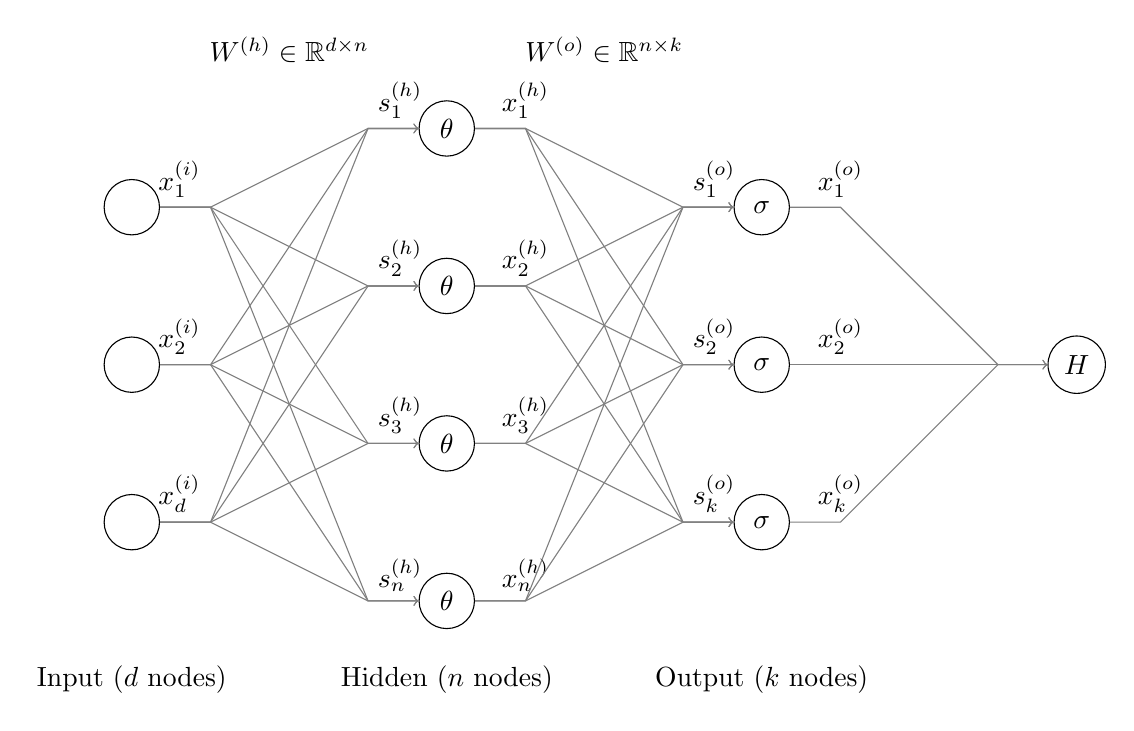
\begin{tikzpicture}[->,draw=black!50]
\tikzstyle{neuron}=[circle,draw=black,minimum size=20pt];

\foreach \i in {1,2,3} {
    \node [neuron] (xi\i) at (1, -2*\i) {};
    \coordinate (xi\i-) at (2, -2*\i);
    \node [above left] at (xi\i-) {$x_{\ifthenelse{\i=3}{d}{\i}}^{(i)}$};
}

\foreach \i in {1,2,3,4} {
    \node [neuron] (xh\i) at (5, -2*\i+1) {$\theta$};
    \coordinate (xh\i-) at (6, -2*\i+1);
    \coordinate (-xh\i) at (4, -2*\i+1);
    \node [above] at (xh\i-) {$x_{\ifthenelse{\i=4}{n}{\i}}^{(h)}$};
    \node [above right] at (-xh\i) {$s_{\ifthenelse{\i=4}{n}{\i}}^{(h)}$};
}

\foreach \i in {1,2,3} {
    \node [neuron] (xo\i) at (9, -2*\i) {$\sigma$};
    \coordinate (xo\i-) at (10, -2*\i);
    \coordinate (-xo\i) at (8, -2*\i);
    \node [above] at (xo\i-) {$x_{\ifthenelse{\i=3}{k}{\i}}^{(o)}$};
    \node [above right] at (-xo\i) {$s_{\ifthenelse{\i=3}{k}{\i}}^{(o)}$};
}

\node [neuron] (h) at (13, -4) {$H$};
\coordinate (-h) at (12,-4);

\foreach \i in {1,2,3} {
    \foreach \j in {1,2,3,4}
        \draw [->] (xi\i) -- (xi\i-) -- (-xh\j) -- (xh\j);
}

\foreach \i in {1,2,3,4} {
    \foreach \j in {1,2,3}
        \draw [->] (xh\i) -- (xh\i-) -- (-xo\j) -- (xo\j);
}

\foreach \i in {1,2,3} {
    \draw [->] (xo\i) -- (xo\i-) -- (-h) -- (h);
}

\node at (3,0) {$W^{(h)} \in \mathbb{R}^{d \times n}$};
\node at (7,0) {$W^{(o)} \in \mathbb{R}^{n \times k}$};

\node at (1,-8) {Input ($d$ nodes)};
\node at (5,-8) {Hidden ($n$ nodes)};
\node at (9,-8) {Output ($k$ nodes)};

\end{tikzpicture}

    \caption{Architecture of the Neural Network.}
    \label{fig:nn-arch}
\end{figure}


The gradient of the loss with respect to the outer layer weights and biases can be found by:
\begin{align*}
\parder{L}{W_{i,j}^{(o)}} &= \parder{L}{s_j^{(o)}} \cdot \parder{s_j^{(o)}}{W_{i,j}^{(o)}} = \parder{L}{s_j^{(o)}} \cdot x_i^{(h)}, \\
\parder{L}{b_j^{(o)}} &= \parder{L}{s_j^{(o)}} \cdot \parder{s_j^{(o)}}{b_j} = \parder{L}{s_j^{(o)}}.
\end{align*}

Denote $\parder{L}{s_j^{(o)}}$ as $\delta_j^{(o)}$, we have

\begin{equation}
\label{eqn:dl_dwo}
\parder{L}{W_{i,j}^{(o)}} = \delta_j^{(o)} x_i^{(h)},
\end{equation}

\begin{equation}
\label{eqn:dl_dbo}
\parder{L}{b_j^{(o)}} = \delta_j^{(o)}.
\end{equation}

where $\delta_j^{(o)} = x_j^{(o)} - y_j$ (from \textbf{Equation (\ref{eqn:grad_cesoftmax})}).

\bigskip

The matrix form of \textbf{Equation (\ref{eqn:dl_dwo})} and \textbf{Equation (\ref{eqn:dl_dbo})} is:

\begin{equation}
\label{eqn:m_dl_dwo}
\parder{L}{\textbf{W}^{(o)}} = \textbf{x}^{(h)} \delta^{(o)},
\end{equation}

\begin{equation}
\label{eqn:m_dl_dbo}
\parder{L}{\textbf{b}^{(o)}} = \delta^{(o)}.
\end{equation}

where 
\begin{equation}
  \label{eqn:m_delta_o}
  \delta^{o} = \textbf{x}^{(o)} - \textbf{y}.
\end{equation}

Next we solve for the derivatives for the hidden layer. The gradient of the loss with respect to the hidden layer weights can be found by:

\begin{align*}
\parder{L}{W_{i,j}^{(h)}} &= \parder{L}{s_j^{(h)}} \cdot \parder{s_j^{(h)}}{w_{i,j}^{(h)}}
= \parder{L}{s_j^{(h)}} \cdot x_i^{(i)}, \\
&= \parder{L}{x_j^{(h)}} \cdot \parder{x_j^{(h)}}{s_j^{(h)}} \cdot x_i^{(i)}
= \parder{L}{x_j^{(h)}} \cdot \theta'(s_j^{(h)}) \cdot x_i^{(i)},
\end{align*}

where $\theta(\cdot)$ is the ReLU activation function in the hidden layer, and

\begin{equation}
\label{eqn:drelu}
\theta'(z) = \begin{cases} 1 &, z > 0 \\ 0 &, \text{otherwise} \end{cases}.
\end{equation}

Since we have \begin{align*}
\parder{L}{x_j^{(h)}} &= \sum_k \Big( \parder{L}{s_k^{(o)}} \cdot \parder{s_k^{(o)}}{x_j^{(h)}} \Big)
= \sum_k \Big( \delta_k^{(o)} \cdot W_{j, k}^{(o)} \Big),
\end{align*}

Let $\delta_j^{(h)}$ denote $\parder{L}{s_j^{(h)}}  = \parder{L}{x_j^{(h)}} \cdot \theta'(s_j^{(h)}) = \sum_k \big( \delta_k^{(o)} \cdot W_{j, k}^{(o)} \big) \cdot \theta'(s_j^{(h)})$, then

\begin{equation}
\label{eqn:dl_dwh}
\parder{L}{W_{i,j}^{(h)}} = \delta_j^{(h)} x_i^{(i)}.
\end{equation}

Similarly, the gradient of the loss with respect to the hidden layer bias is

\begin{equation}
\label{eqn:dl_dbh}
\parder{L}{b_{j}^{(h)}} = \delta_j^{(h)} \parder{s_j^{h}}{b_j^{h}}
= \delta_j^{(h)}.
\end{equation}

 \textbf{Equation (\ref{eqn:dl_dwh})} and \textbf{Equation (\ref{eqn:dl_dbh})} can be written in matrix form as:

\begin{equation}
\label{eqn:m_dl_dwh}
\parder{L}{\textbf{W}^{(h)}} = \textbf{x}^{(i)} \delta^{(h)},
\end{equation}

\begin{equation}
\label{eqn:m_dl_dbh}
\parder{L}{\textbf{b}^{(h)}} = \delta^{(h)},
\end{equation}

where
\begin{equation}
\label{eqn:m_delta_h}
\delta^{(h)} = \delta^{(o)} {\textbf{W}^{(o)}}^\intercal \cdot \theta'(s^{h}).
\end{equation}

\bigskip
\subsection{Learning}

A neural network is constructed and trained according to the required specifications, and the detailed implementation can be referred to in the source code submitted separately. Due to memory constraints, Stochastic Gradient Descent is utilized here instead of Full Gradient Descent.
With batch size = 100, the neural network is trained for 200 epochs with a hidden unit size of 1000, the resulting loss and accuracy curves for the training, validation and test data sets are shown in \textbf{Figure \ref{fig:1-3}}. 

As observed in the figure, the learning process appears to be correctly implemented, since the overall trend of the training loss is monotonically decreasing, corresponding to the training accuracy increasing with increased epochs. The local roughness in the curves can be contributed to the fact that Stochastic Gradient Descent is implemented here. It can also be inferred from the figure that this model starts to overfit the data after around 53 epochs, since the test and the validation losses start to increase even though the test loss continues to decrease.
\begin{figure}[!htb]
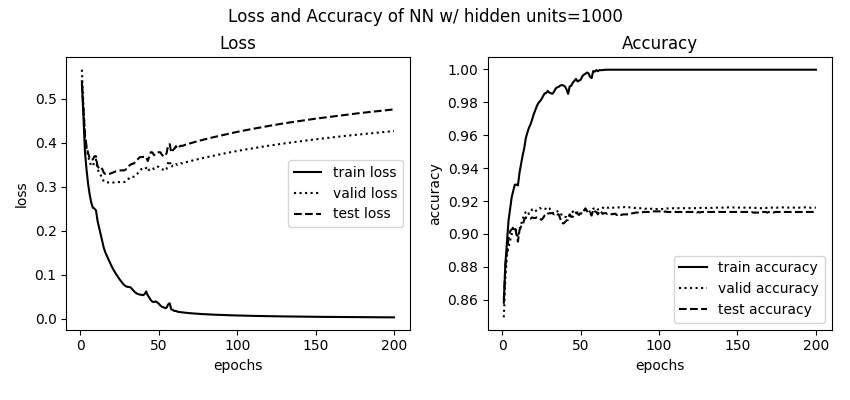
\includegraphics[width=0.95\linewidth]{images/a2/1.3/loss.png}
\caption{Loss(left) and accuracy(right) curves for training, validation and test data sets, of the neural network with 1000 hidden units trained for 200 epochs. Batch size = 100 and learning rate $\alpha = 1 \times 10^{-5}$ is used for Stochastic Gradient Descent.}  \label{fig:1-3}
\end{figure}

\bigskip
\subsection{Hyperparameter Investigation}
\subsubsection{Number of hidden units}

To investigate the effects of the number of hidden units on the classification accuracy of neural networks, three different hidden unit sizes [100, 500, 2000] are used in the model instead of 1000 from the previous part. \textbf{Figure \ref{fig:1-4}} shows the resulting training and test accuracy curves.

As shown in the figure, larger hidden unit sizes tend to achieve higher accuracy and converge faster in terms of training accuracy. Although after sufficient number of epochs, the final training accuracy that different hidden unit sizes can reach appear to become about the same, indicating the ultimate accuracy the neural network can achieve in fitting the training set. 

In the case of test accuracy, larger hidden unit sizes appear to achieve better accuracy. Specifically, the model with 100 hidden units has significantly lower test accuracy than models with 500 and 2000 hidden units, indicating that for this problem, the model with less hidden units does not have enough complexity to well generalize the model to unseen data, i.e. underfitting.
Generally speaking, more hidden units allow for higher complexity in the model which may contribute to the model with better generalization to test data. 

\begin{figure}[!htb]
\hspace*{-2cm}
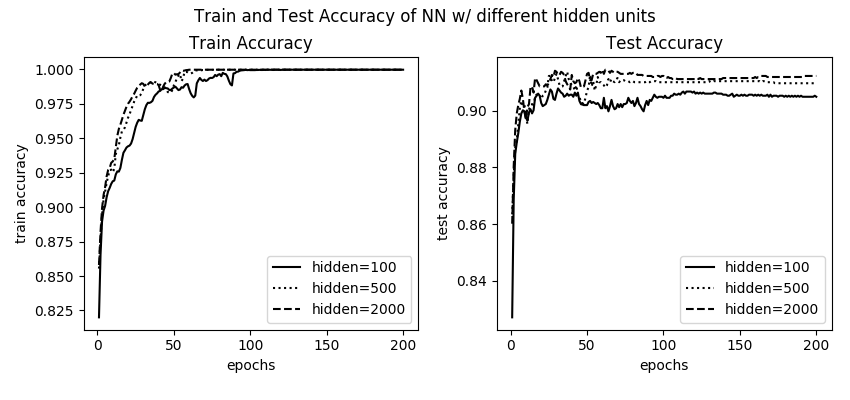
\includegraphics[width=1.2\linewidth]{images/a2/1.4/accuracy.png}
\caption{Training(left) and test(right) accuracy curves for neural networks with 100, 500 and 2000 hidden units respectively.}\label{fig:1-4}
\end{figure}

\bigskip
\subsubsection{Early stopping}

From \textbf{Figure \ref{fig:1-3}} we find that the validation and test accuracies become stabilized after around 50 epochs. The test accuracy reaches its peak at about 53 epochs. After that, both validation loss and test loss start to increase even though the training loss is continuously decreased. This suggests the sign of overfitting and signifies a reasonable early stopping point can be chosen at epoch 53. The classification accuracy data after epoch 53 is listed below:

\begin{itemize}
    \item Training Accuracy: 99.73\%
    \item Validation Accuracy: 91.47\%
    \item Test Accuracy: 91.56\%
\end{itemize}
\bigskip
\section{Neural Networks in Tensorflow}

\subsection{Model implementation}
In this part, a Convolutional Neural Network is implemented in Tensorflow for image recognition. The network architecture is implemented as required and a snippet of Python code is given below:   

\begin{minted}
[
frame=lines,
framesep=2mm,
baselinestretch=1.0,
fontsize=\footnotesize,
]{python}
  def build_graph(self, image_size=28, num_of_class=10, conv_params=(3, 32, 1),
                  pool_size=2, alpha=1e-4):
    """Build a convolutional neuron network.

    :param image_size: The width/height of the input image. Image must be a square
                       with size of (image_size, image_size).
    :param num_of_class: Number of output classes.
    :param conv_params: A 3-element tuple
    , specifying (kernel_size, num_of_filters,
                        stride) for conv layer.
    :param pool_size: Size of max_pool layer.
    :param alpha: Learning rate.
    """
    with tf.name_scope('input'):
      # 1. Input layer
      self.X = tf.placeholder(tf.float32, shape=(None, image_size, image_size),
                              name='X')
      X_reshaped = tf.reshape(self.X, shape=(-1, image_size, image_size, 1), 
                              name='X_reshaped')

      # Target
      self.y = tf.placeholder(tf.int64, shape=(None,), name='y')
      y_onehot = tf.one_hot(self.y, num_of_class)

    with tf.name_scope('conv_pool'):

      # 2. Conv layer
      kernel_size, num_of_filters, stride = conv_params
      W_conv = tf.get_variable('W_conv', dtype=tf.float32,
                               shape=(kernel_size, kernel_size, 1, num_of_filters),
                               initializer=tf.contrib.layers.xavier_initializer())
      b_conv = tf.get_variable('b_conv', shape=(num_of_filters,),
                               initializer=tf.contrib.layers.xavier_initializer())
      conv = tf.nn.conv2d(X_reshaped, W_conv, strides=(1, stride, stride, 1),
                          padding='SAME') + b_conv

      # 3. ReLU activation
      h_conv = tf.nn.relu(conv)

      # 4. Bath normalization
      h_mean, h_var = tf.nn.moments(h_conv, axes=[0])
      batch_norm = tf.nn.batch_normalization(h_conv, h_mean, h_var,
                                             None, None, 1e-9)

      # 5. Max pooling
      h_pool = tf.nn.max_pool(batch_norm, ksize=[1, pool_size, pool_size, 1],
                              strides=[1, pool_size, pool_size, 1],
                              padding='SAME', name='h_pool')

      # 6. Flatten
      feature_count = int(image_size * image_size / pool_size / pool_size *
                          num_of_filters)
      h_flat = tf.reshape(h_pool, shape=[-1, feature_count], name='h_flat')

    with tf.name_scope('fc1'):

      # 7. FC1 layer
      fc_size = image_size * image_size
      W_fc1 = tf.get_variable('W_fc1', shape=(feature_count, fc_size),
                              dtype=tf.float32,
                              initializer=tf.contrib.layers.xavier_initializer())
      b_fc1 = tf.get_variable('b_fc1', shape=(fc_size,), dtype=tf.float32,
                              initializer=tf.contrib.layers.xavier_initializer())
      h_fc1 = tf.matmul(h_flat, W_fc1) + b_fc1

      # Dropout layer
      self.p_dropout = tf.placeholder(tf.float32, shape=(), name='p_dropout')
      h_fc1 = tf.nn.dropout(h_fc1, keep_prob=self.p_dropout)

      # 8. ReLU
      h_fc1 = tf.nn.relu(h_fc1)

    with tf.name_scope('fc2'):
      # 9. FC2 layer
      W_fc2 = tf.get_variable('W_fc2', shape=(fc_size, num_of_class), 
                              dtype=tf.float32,
                              initializer=tf.contrib.layers.xavier_initializer())
      b_fc2 = tf.get_variable('b_fc2', shape=(num_of_class,), dtype=tf.float32,
                              initializer=tf.contrib.layers.xavier_initializer())
      h_fc2 = tf.matmul(h_fc1, W_fc2) + b_fc2

    with tf.name_scope('output'):

      # 10. Softmax
      h_softmax = tf.nn.softmax(h_fc2)

    # 11. Cross Entropy Loss
    self.loss = tf.reduce_mean(tf.nn.softmax_cross_entropy_with_logits_v2(
      labels=y_onehot, logits=h_fc2))
    
    # L2 regularization
    self.l2_lambda = tf.placeholder(tf.float32, shape=(), name='l2_lambda')
    reg = self.l2_lambda * (tf.nn.l2_loss(W_conv) + tf.nn.l2_loss(W_fc1) +
          tf.nn.l2_loss(W_fc2))
    self.loss = self.loss + reg

    # Optimizer
    self.opt_op = tf.train.AdamOptimizer(learning_rate=alpha).minimize(self.loss)

    # Predict
    self.predict = tf.argmax(h_softmax, 1)
    self.accuracy = tf.reduce_mean(
      tf.cast(tf.equal(self.predict, self.y), tf.float32)
    )

\end{minted}

\subsection{Model Training}

The Convolutional Neural Network is trained using SGD for a batch size of 32, 50 epochs, and the learning rate $\alpha$  is set to $10^{-4}$ in the Adam optimizer. The training, validation and test loss and accuracy curves are plotted in \textbf{Figure \ref{fig:2-2}}. As shown in the figure, the training accuracy very quickly converges to nearly 1 after the training commences. The validation and test accuracies appear to stablize after around 20 epochs. After that, validation and test losses start increasing even though the training loss keeps decreasing, indicating the occurrence of overfitting.  

\begin{figure}[!htb]
\hspace*{-2cm}
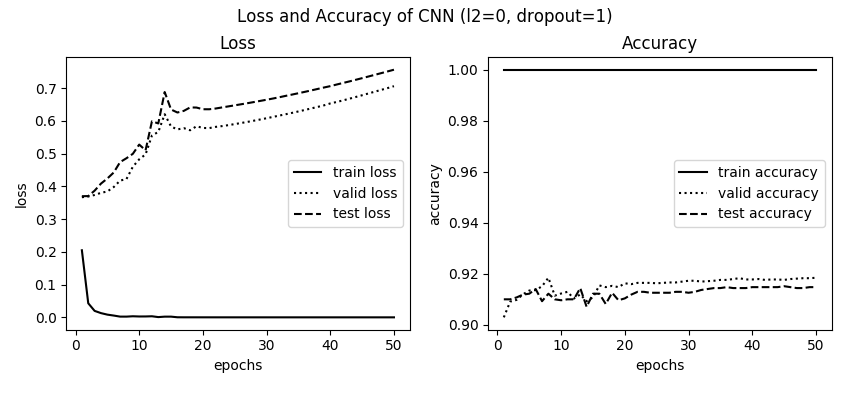
\includegraphics[width=1.2\linewidth]{images/a2/2.2/loss.png}
\caption{Training, validation and test loss(left) and accuracy(right) curves for the Convolutional Neural Network with no regularization or dropout.}\label{fig:2-2}
\end{figure}

\bigskip
\subsection{Hyperparameter Investigation}

\subsubsection{L2 Normalization}

L2 regularization is performed on the weights in the model using three different weight decay coefficients $\lambda = [0.01, 0.1, 0.5]$. The training, validation and test accuracy curves under various $\lambda$  settings are presented in \textbf{Figure \ref{fig:2-3-1}}. The final accuracy results after 50 epochs are summarized in \textbf{Table \ref{tab:2-3-1}}.

As we can see from the table, $\lambda = 0.1$ achieves the highest final validation and test accuracy when compared to the others, which indicates that it is the better choice out of the three $\lambda$ values. When  $\lambda=0.5$, the final training, validation and test accuracy scores are significantly lower than the other two cases. 

This shows the bias-variance trade off.
If $\lambda$ is too large, it will excessively penalize the weights, resulting in high bias and low variance, leading to under-fitting of the model. Conversely, when $\lambda = 0.01$, the training accuracy reaches its highest 100\%, but the validation and test accuracies are lower than those with $\lambda=0.1$. This is consistent with the fact that small $\lambda$ can result in low bias and high variance in the model, which may possibly cause overfitting of the model.


\begin{table}[!htb]
\center
\begin{tabular}{|l|l|l|l|l|l|}
\hline
weight decay coefficient $\lambda$ & training accuracy & validation accuracy   & test accuracy     \\ \hline
0.01   & 100\%  & 92.37\% & 92.11\%  \\ \hline
0.1    &93.75\%  & 92.50\% & 92.69\%  \\ \hline
0.5    & 87.5\%  & 89.02\% & 90.12\%  \\ \hline

\end{tabular}
\caption{The final training, validation and test accuracies after 50 epochs under three different weight decay coefficient settings $\lambda=[0.01, 0.1, 0.5]$.}
\label{tab:2-3-1}
\end{table}





\begin{figure}[!htb]
\hspace*{-2cm}
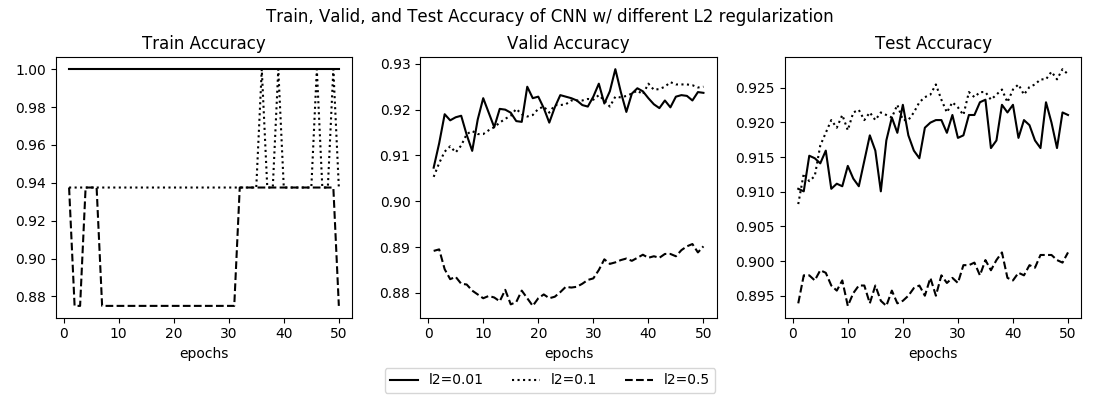
\includegraphics[width=1.2\linewidth]{images/a2/2.3-1/accuracy.png}
\caption{The training, validation and test accuracy curves under three different weight decay coefficient settings $\lambda=[0.01, 0.1, 0.5]$.}\label{fig:2-3-1}
\end{figure}

\subsubsection{Dropout}
To investigate the influence of dropout on model performance, three probability values $p=[0.9, 0.75, 0.5]$ are applied to the dropout layer in the model. The training, validation and test accuracy curves are plotted in \textbf{Figure \ref{fig:2-3-2}}. After examining the figure, we can see that higher dropout probability tends to converge faster in terms of training accuracy, while the final training accuracies reached under different probability scenarios are all very close to 1. Meanwhile, $p=0.5$ generally achieves the best validation and test accuracies among the three, followed by  $p=0.9$, with  $p=0.75$ having the poorest overall validation and test classification performance. This confirms that $p=0.5$ is the better choice for dropout probability in order to control overfitting and enhance model accuracy performance.  

\begin{figure}[!htb]
\hspace*{-2cm}
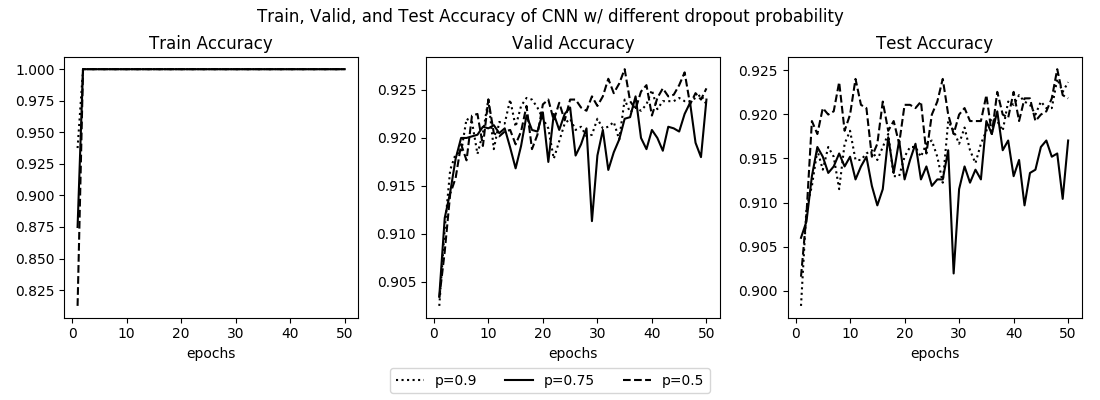
\includegraphics[width=1.2\linewidth]{images/a2/2.3-2/accuracy.png}
\caption{Training, validation and test accuracy curves with three different dropout probabilities  $p=[0.9, 0.75, 0.5]$.}\label{fig:2-3-2}
\end{figure}


\newpage

\end{document}